\chapter{Cálculo del \textit{Skeleton} por Adelgazamiento Topológico Paralelo}
\label{ch:palagyi}

El primer algoritmo implementado para esta tesis fue presentado por Palágyi et al. en \cite{palagyi1999parallel}. Este algoritmo simula la metáfora del incendio de Blum eliminando vóxeles del contorno del objeto hasta transformarlo en su \textit{skeleton}. La secuencia de eliminación no es arbitraria, sino que está determinada por máscaras.

Un vóxel es eliminado si su 26-vecindad calza con alguna máscara, es decir, si satisface cierto patrón de unos y ceros. En general, los algoritmos que siguen una estrategia similar son referidos como ''algoritmos de adelgazamiento topológico'', porque cada operación de eliminación va haciendo más delgado el objeto sin alterar su topología. Esto significa que una condición mínima para las máscaras es que solamente vóxeles simples sean eliminados.

\begin{figure}[H]\centering
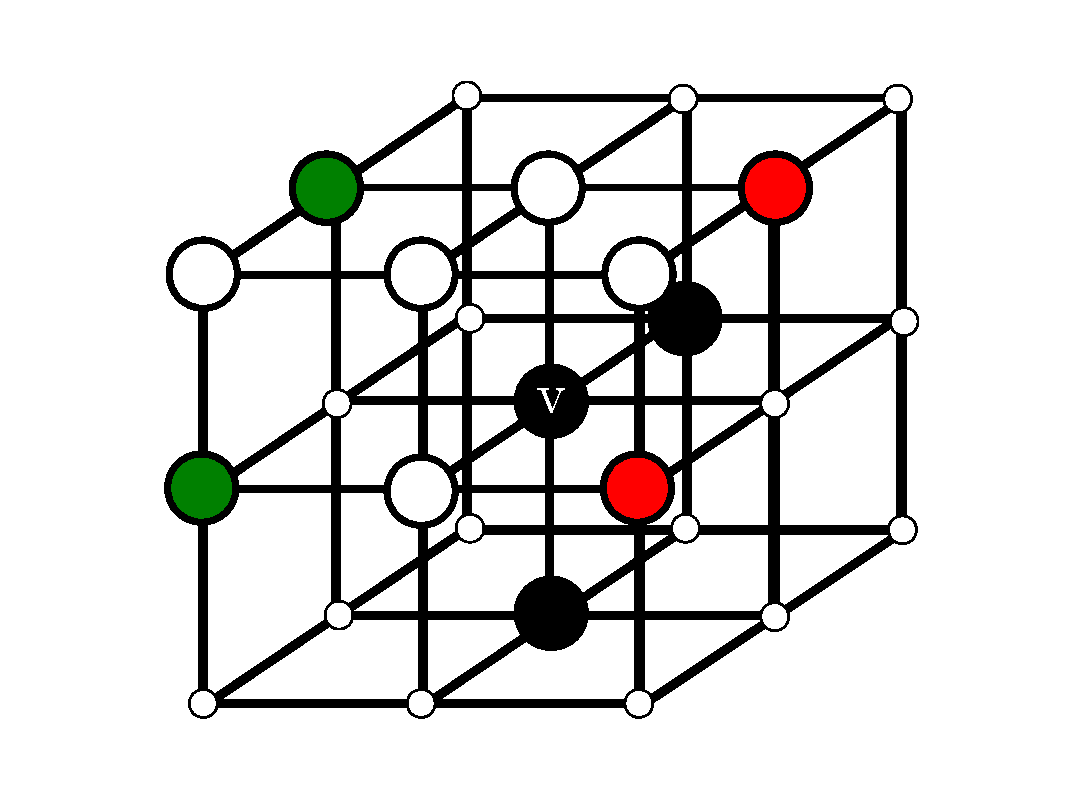
\includegraphics[width=0.5\linewidth]{images/palagyi_mask}
\caption{Ejemplo de máscara usada en este algoritmo}
\label{fig:palagyi_mask}
\end{figure}

Este algoritmo se dice además ''paralelo'' porque todos los vóxeles que calzan con cualquier máscara pueden ser eliminados simultáneamente. Existen otros algoritmos de adelgazamiento llamados ''totalmente paralelos''. La diferencia es que en los algoritmos paralelos a secas las máscaras deben aplicarse varias veces, siguiendo una secuencia fija de direcciones, mientras que en los totalmente paralelos se aplican sin rotarse. La mayoría de los algoritmos de adelgazamiento paralelo usa 6 rotaciones para las máscaras.

Este algoritmo en particular usa 12 rotaciones, reduciendo así el número de máscaras a definir.

\section{Fundamentos teóricos}

De acuerdo a los autores, el diseño de las máscaras se hizo con cuatro objetivos en mente, que tienen que ver con las propiedades que este algoritmo busca satisfacer.

\begin{enumerate}
\item Las máscaras solamente eliminan vóxeles simples. Esto es claro al observar que ninguna máscara desconecta el objeto ni crea un agujero.
\item La centralidad viene dada gracias a la erosión multidireccional. Las máscaras se muestran en la Figura \ref{fig:palagyi_all_masks} orientadas en la primera de las 12 rotaciones. El cubo de la Figura \ref{fig:palagyi_orientations} representa una máscara orientada en la primera rotación. El orden de las rotaciones, etiquetadas según las caras que apuntan hacia arriba y adelante en esa figura, debe ser: US, NE, WD, ES, UW, ND, SW, UN, UD, NW, UE y SD.

\begin{figure}[H]\centering
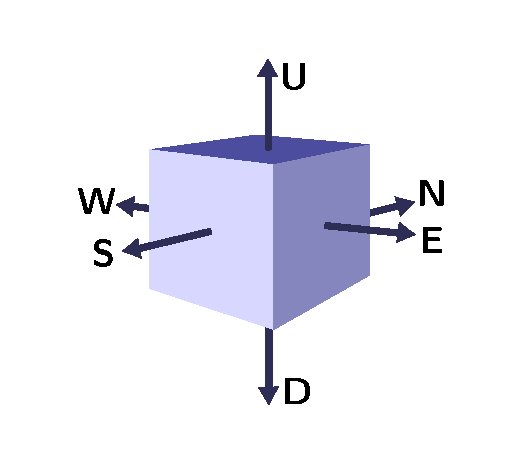
\includegraphics[width=0.5\linewidth]{images/palagyi_orientations}
\caption{asdasd}
\label{fig:palagyi_orientations}
\end{figure}

\item Las máscaras buscan preservar los puntos de término significativos. Esto es difícil sin criterios de carácter más global. Como se verá en los resultados, el \textit{skeleton} producido resulta con menos vóxeles de término de los esperados.

\item El grado de delgadez del \textit{skeleton} debe ser ``máximo''.

\end{enumerate}

\begin{figure}[H]\centering
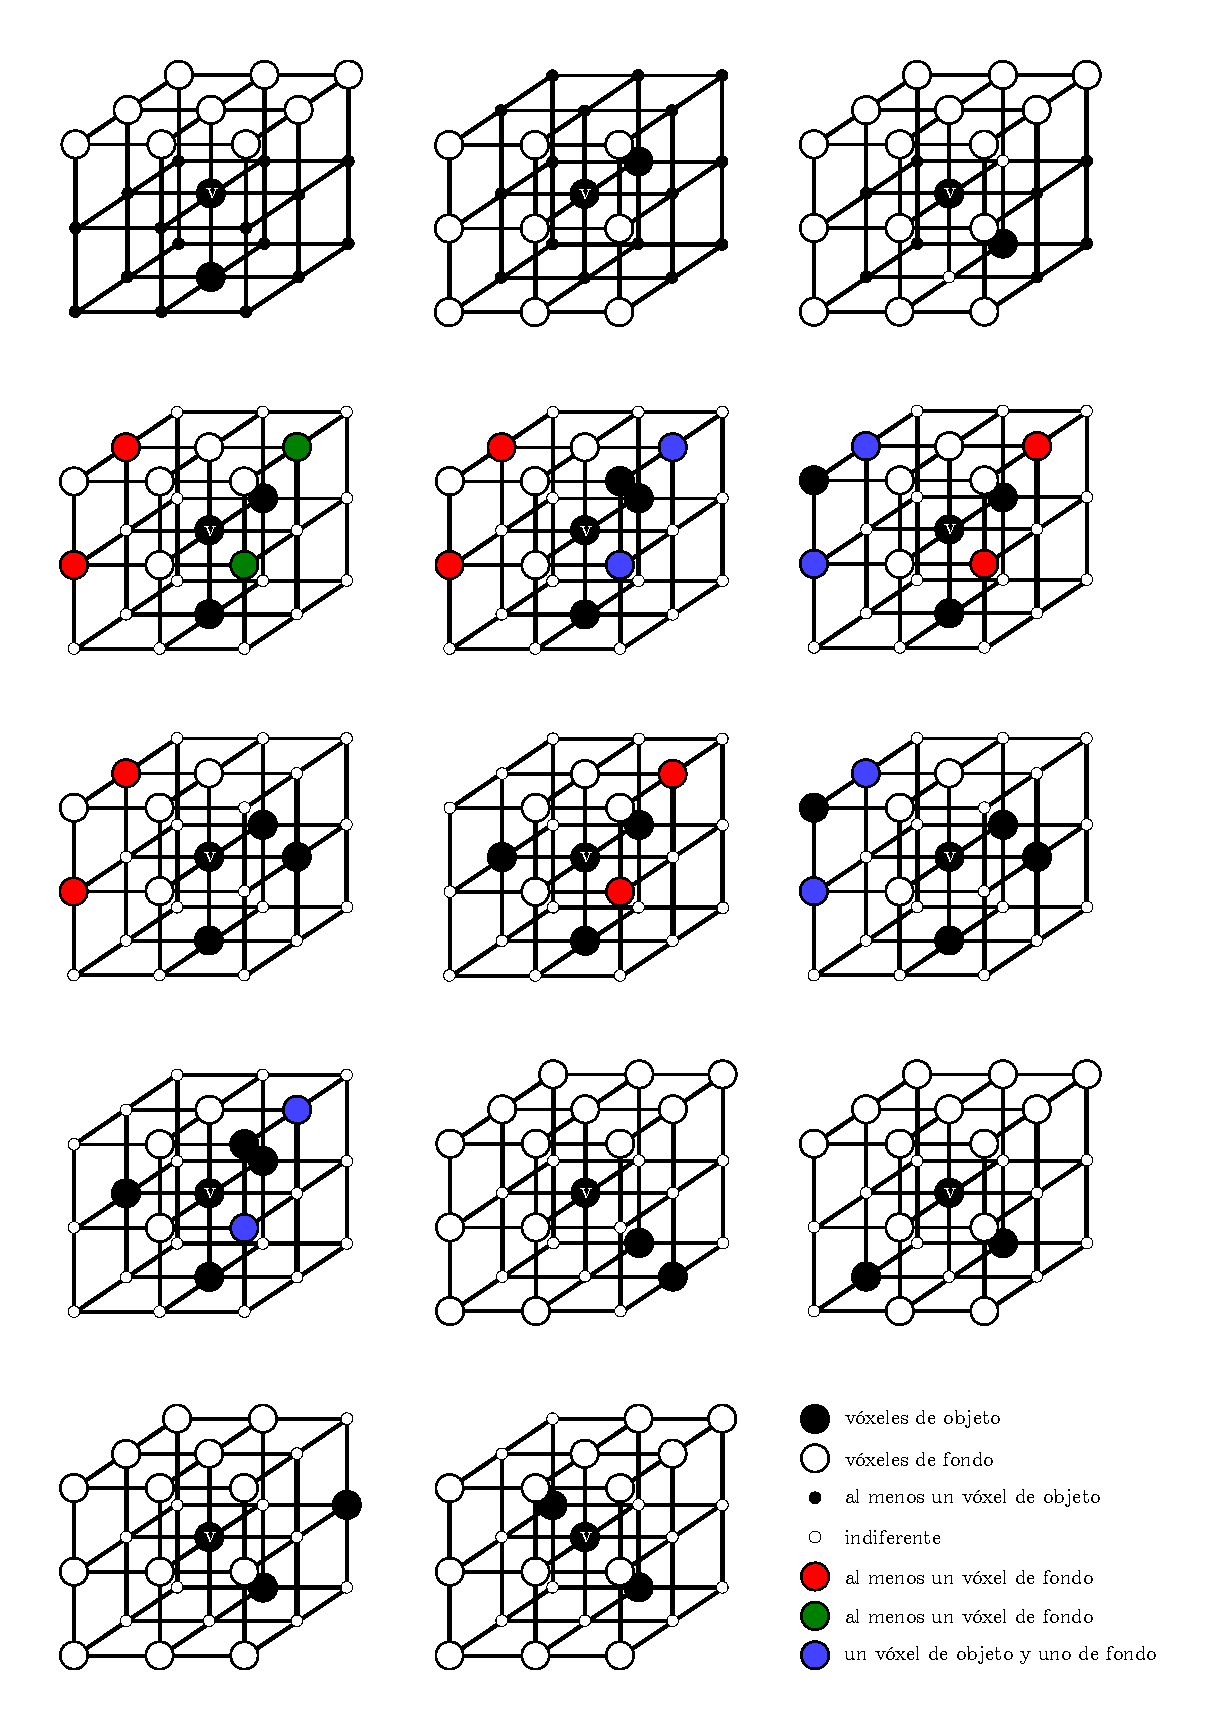
\includegraphics[width=0.95\linewidth]{images/palagyi_all_masks}
\caption{Las 14 máscaras usadas en este algoritmo, en su primera rotación (US)}
\label{fig:palagyi_all_masks}
\end{figure}

\section{Visión general del algoritmo}

\algdef{SE}[DOWHILE]{Do}{doWhile}{\algorithmicdo}[1]{\algorithmicwhile\ #1} %do-while definicion jeje no se por que funciona

\begin{algorithm}[H]
\caption{Adelgazamiento topológico paralelo de Palágyi et al.}
\label{alg:thinning}
\begin{algorithmic}[1]
\Function{AdelgazamientoTopologicoParalelo}{$I$}
	\State $mascaras \gets InicializarMascaras()$
	\State $rotaciones \gets InitcializarRotaciones()$
	\State $skel \gets I$
  	\Do
    	\State $prevSkel \gets skel$
        \State $eliminables \gets Zeros(Size(skel))$
        \ForAll {$r \in rotaciones$}
    		\ForAll {$m \in mascaras$}
            	\State $mascaraRotada \gets Rotate(m, r)$
        		\State $eliminables \gets eliminables \cup AplicarMascara(mascaraRotada, skel)$
            \EndFor
        \EndFor
        \State $skel \gets skel - eliminables$
  	\doWhile{$prevSkel \neq skel$}
    \State \Return $skel$
\EndFunction
\end{algorithmic}
\end{algorithm}

En resumen, este algoritmo consiste en eliminar vóxeles cuya 26-vecindad calce con alguna de las 14 máscaras, rotadas en cada una de las 12 rotaciones predefinidas, hasta que la aplicación de todas las máscaras en todas las rotaciones no elimine ningún vóxel. Por lo tanto, cada iteración consiste en evaluar $12 \times 14 = 168$ máscaras en la vecindad cada vóxel de la imagen.

\section{Detalles de la implementación}

Este algoritmo se implementó de dos maneras, con el objetivo de asegurar la consistencia de sus resultados. Esto porque se encontró que la principal dificultad en su implementación está en no cometer errores al especificar las máscaras. En principio, como cada máscara tiene 27 valores, es necesario considerar $14 \times 27 = 378$ valores en el código.

Sin embargo, para la primera implementación se quiso usar la operación morfológica \textit{hit-and-miss}, tal como se hace para el algoritmo de adelgazamiento 2D de \cite{jain1995machine}, aprovechando que MATLAB dispone de la operación \textit{hit-and-miss} para imágenes 3D. La operación \textit{hit-and-miss} 3D busca el calce con patrones en la 26-vecindad de un vóxel, pero solamente admite máscaras cuyos valores calcen estrictamente con 1, estrictamente con 0, o con cualquier valor. Es decir, no es posible especificar directamente las condiciones de calce de las máscaras que involucran solo a cierto subconjunto de vóxeles (como, por ejemplo, que al menos un vóxel de entre los marcados con rojo en la Figura \ref{fig:palagyi_split} sea de fondo). Debido a esto, para poder usar \textit{hit-and-miss} varias de las 14 máscaras debieron ser divididas, totalizando 63 máscaras. Esto aumentó la posibilidad de error, puesto que ahora debieron escribirse $63 \times 27 = 1701$ valores.

\begin{figure}[H]\centering
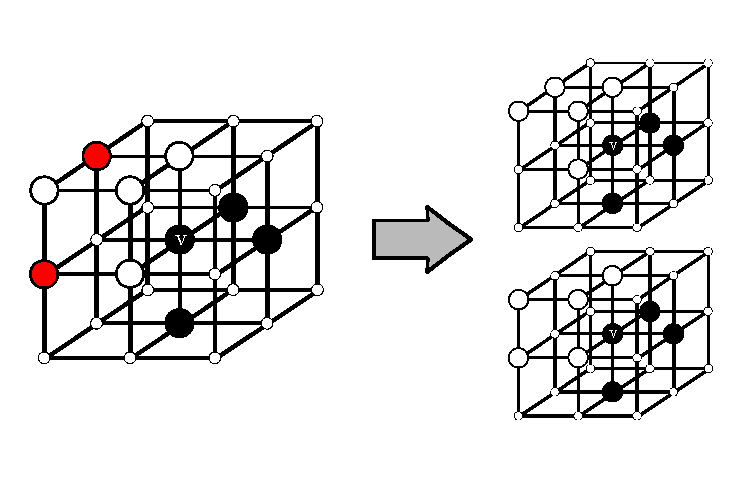
\includegraphics[width=0.6\linewidth]{images/palagyi_split}
\caption{Ejemplo de máscara que debe dividirse para poder usar \textit{hit-and-miss}}
\label{fig:palagyi_split}
\end{figure}

En vista de que resultaba muy difícil asegurar la correctitud del código de la primera implementación, se optó por programar el algoritmo una segunda vez, siguiendo principios distintos. Esta segunda implementación adopta las sugerencias que aparecen en \cite{palagyi1999parallel}.

Para cada máscara se construye una función booleana que recibe la 26-vecindad del vóxel que se quiere revisar. Para usar operadores booleanos en el cuerpo de esta función, los vóxeles de objeto se consideran \textit{true} y los vóxeles de fondo \textit{false}. Cada vóxel en la 26-vecindad es identificado con una etiqueta según su posición, como se muestra en la Figura \ref{fig:palagyi_numbers}.

\begin{figure}[H]\centering
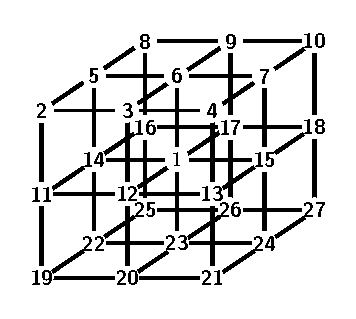
\includegraphics[width=0.4\linewidth]{images/palagyi_numbers}
\caption{Etiquetado de la 26-vecindad}
\label{fig:palagyi_numbers}
\end{figure}

Luego, a modo de ejemplo, el calce de un vóxel $v$ (cuya etiqueta en el cuerpo de la función es $v_1$) con la máscara de la Figura \ref{fig:palagyi_split} puede ser revisado usando la función:

\begin{equation*}
F_{M7}(v, I) = v_1 \land v_{15} \land v_{17} \land v_{23} \land \neg(v_2 \lor v_3 \lor v_6) \land \neg(v_5 \land v_{11})
\end{equation*}

Al no usar funciones nativas, ejecutar el algoritmo programado de acuerdo a este enfoque tiene mayor costoso computacional en MATLAB. La ventaja es que las máscaras a ingresar se mantienen en 14, reduciendo la probabilidad de errores.

A fin de cuentas, ambas implementaciones produjeron resultados idénticos para las figuras de prueba, certificando su correctitud.

\section{Resultados}

\begin{figure}[H]\centering
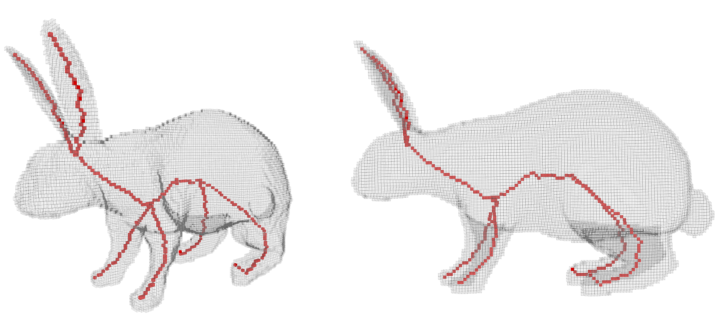
\includegraphics[width=0.95\linewidth]{images/palagyi_rabbit_demo}
\caption{Por algo puse estos conejos}
\label{fig:palagyi_rabbit_demo}
\end{figure}

\begin{figure}[H]\centering
\includegraphics[width=1\linewidth]{images/palagyi_test_models}
\caption{Resultados del algoritmo de Palágyi et al. para las imágenes de prueba}
\label{fig:palagyi_test_models}
\end{figure}
